%template1.tex
%The following LaTeX source file represents the simplest kind of slide presentation; no overlays, no included graphics. Substitute your favorite style for ``pascal''. To create the PDF file template1.pdf, (1) be sure to use the prosper class, then (2) execute the command latex template1.tex, and (3) the command dvipdf template1.dvi.

%%%%%%%%%%%%%%%%%%%%%%%%%%%%%%% template1.tex %%%%%%%%%%%%%%%%%%%%%%%%%%%%%%%%%%%
\documentclass[a4paper,blends,pdf,colorBG,slideColor]{prosper}
% definitions for slides for CSC544
% Lutz Hamel, (c) 2007

\hypersetup{pdfpagemode=FullScreen}

\usepackage{amssymb}
\usepackage{latexsym}
\usepackage{amsmath}
%\usepackage[usenames]{color}
\usepackage{xypic}


\newcommand{\term}[1]{\ensuremath{\mbox{\bf #1}}}
\newcommand{\nonterm}[1]{\ensuremath{\mbox{#1}}}
\newcommand{\ifstmt}[3]{\ensuremath{{\bf if}\; {#1}\;{\bf then}\;{#2}\;{\bf else}\;{#3}\;\term{end}}}
\newcommand{\whilestmt}[2]{\ensuremath{{\bf while}\; {#1}\;{\bf do}\;{#2}\; \term{end}}}
\newcommand{\funcstmt}[3]{\ensuremath{{\bf fun}\; {#1}\; {\bf is}\; {#2} \; {\bf return}\; {#3}}}
\newcommand{\syntaxset}[1]{\ensuremath{\mbox{\bf #1}}}
\newcommand{\orbar}{\;|\;}
\newcommand{\bs}[1]{\begin{slide}{#1}\ptsize{8}}
\newcommand{\es}{\end{slide}}
\newcommand{\co}{\,\colon\;}
\newcommand{\pair}[2]{\ensuremath{\langle {#1}, {#2} \rangle}}
\newcommand{\encode}[1]{\ensuremath{\langle {#1} \rangle}}
\newcommand{\mytab}{\makebox[.15in]{}}
%\newcommand{\abs}[1]{{\mid{#1}\mid}}
\newcommand{\abs}[1]{{|{#1}|}}
\newcommand{\ol}[1]{\overline{#1}}

\newcommand{\qaccept}{\ensuremath{q_{\mbox{\tiny accept}}}}
\newcommand{\qreject}{\ensuremath{q_{\mbox{\tiny reject}}}}
\newcommand{\accept}{{\em accept}}
\newcommand{\reject}{{\em reject}}

\newcommand{\machine}[1]{
	\begin{quote}
	{#1}
	\end{quote}
	}

\newcommand{\fdef}[1]{
	\begin{center}
	\fbox{
	\begin{minipage}{3.5in}
	{\bf Definition:}
	{#1}
	\end{minipage}
	}
	\end{center}
	}

\newcommand{\ftheorem}[1]{
	\begin{center}
	\fbox{
	\begin{minipage}{3.5in}
	{\bf Theorem:}
	{#1}
	\end{minipage}
	}
	\end{center}
	}

\newcommand{\flemma}[1]{
	\begin{center}
	\fbox{
	\begin{minipage}{3.5in}
	{\bf Lemma:}
	{#1}
	\end{minipage}
	}
	\end{center}
	}


\newcommand{\fframe}[1]{
	\begin{center}
	\fbox{
	\begin{minipage}{3.5in}
	{#1}
	\end{minipage}
	}
	\end{center}
	}

\newcommand{\nframe}[1]{
	\begin{center}
	\begin{minipage}{3.5in}
	{#1}
	\end{minipage}
	\end{center}
	}

\begin{document}
\bs{Regular Languages}

\vspace{.5in}

\framebox{{\bf Definition:} A language is called a {\bf regular language} if some finite
automaton recognizes it}
\es

\bs{Regular Operations}
{\bf Definition:} Let $A$ and $B$ be regular languages, we define the following
operations:
\begin{description}
\item[Union:] $A \cup B = \{ x \mid x \in A \mbox{ or } x\in B\}$.
\item[Concatenation:] $A \circ B = \{ xy \mid x\in A \mbox{ and } y \in B\}$.
\item[Star (Kleene Closure):] $A^* =  \{ x_1 x_2 \ldots x_k \mid k \ge 0 \mbox{ and each } x_i \in A\}$.
\end{description}

\es

\bs{$A \cup B$ is a Regular Language}
{\bf Theorem:} If $A_1$ and $A_2$ are regular languages, then so is $A \cup B$.\footnote{We postpone the
proofs of the other regular operations until we discussed nondeterminism.}

\vspace{2in}
\es

\bs{$A \cup B$ is a Regular Language}
\begin{center}
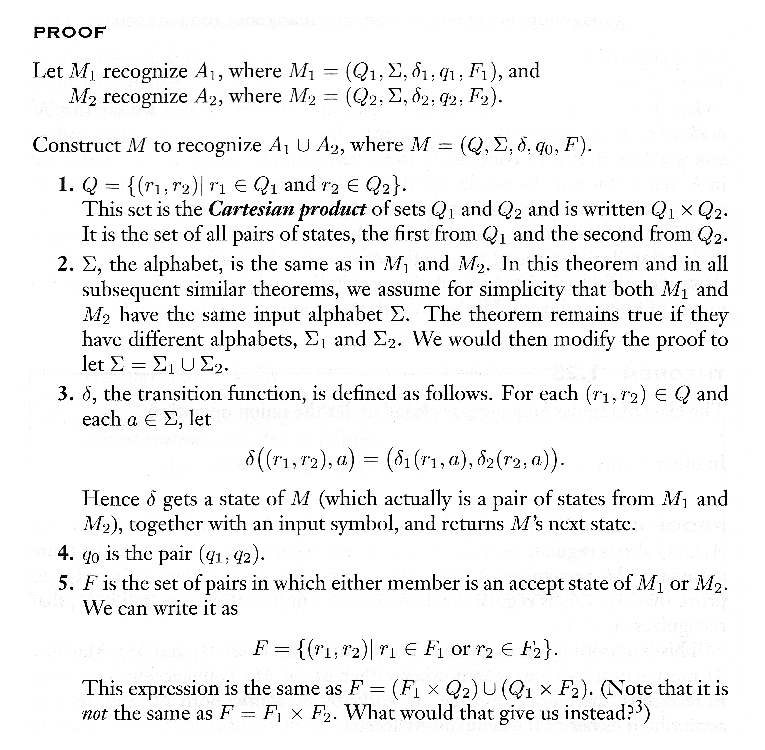
\includegraphics[height=70mm]{images/union-proof.eps}
\end{center}
\es

\bs{Nondeterminism}
Up to now we have only considered machines where, given a state and given an input symbol, the next state is uniquely defined - {\bf\em deterministic machines (DFA)}

However, we could conceive of machines that, given a state and a particular input symbol, have a choice of states to move to - {\bf\em nondeterministic machines (NFA)}

We will see that nondeterminism does not add to the power of the NFA to recognize larger sets of languages, but nondeterminism adds to the expressiveness of the machines, i.e., it is much easier to build a nondeterministic machine for a particular
regular language than a deterministic machine.

\es


\bs{NFA}
{\bf Example:} Let $A$ be the language consisting of all strings over $\Sigma = \{0,1\}$
containing a $1$ in the third position from the end (e.g. $00100,0101,1100\in A$).

DFA:
\begin{center}
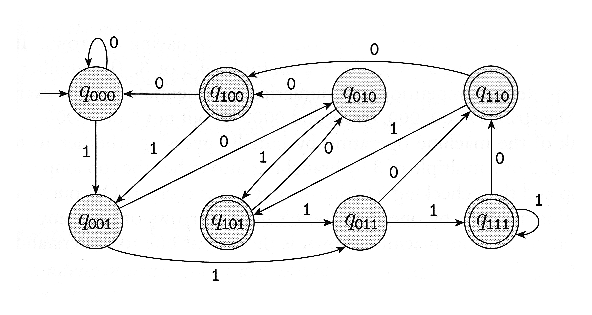
\includegraphics[height=30mm]{images/dfa.eps}
\end{center}

NFA:
\begin{center}
\includegraphics[height=15mm]{images/nfa.eps}
\end{center}

\es

\bs{Computing with NFAs}
\begin{center}
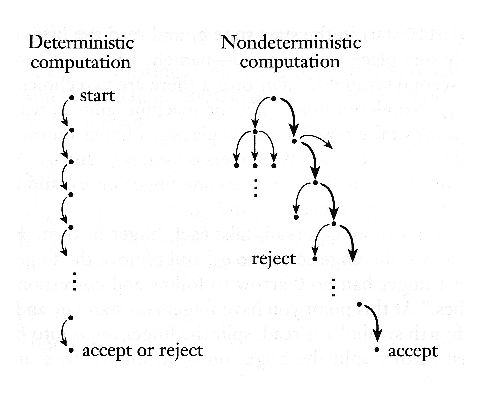
\includegraphics[height=70mm]{images/nfa-comp.eps}
\end{center}
\es

\bs{Computing with NFAs}
{\bf Example:} Consider the computation of the following NFA,
\begin{center}
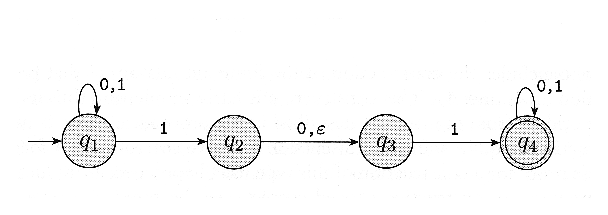
\includegraphics[height=15mm]{images/nfa2.eps}
\end{center}
with input string $s=010110$,
\begin{center}
\includegraphics[height=40mm]{images/nfa2-comp.eps}
\end{center}

\es

\bs{Formal Def. of NFA}

{\bf Definition:} a {\bf {\color{red} nondeterministic} finite automaton} is a 5-tuple $(Q, \Sigma, \delta, q_0, F)$, where
\begin{enumerate}
\item $Q$ is a finite set called the {\bf states},
\item $\Sigma$ is a finite set called the {\bf alphabet},
\item $\delta\co Q \times \Sigma_{\color{red}\epsilon} \rightarrow {\color{red}P(Q)}$ is the {\bf transition function},
\item $q_0 \in Q$ is the {\bf start state}, and
\item $F \subseteq Q$ is the {\bf set of accept states}.
\end{enumerate}

\es

\bs{DFA $\equiv$ NFA}
We say that two machines are {\bf\em equivalent} if they recognize the same language.

\begin{center}
\framebox{{\bf Theorem:} Every NFA has an equivalent DFA.}
\end{center}

{\bf Proof Sketch:} For every NFA we can construct a DFA that simulates it.  We do
so by introducing new states that remove multiple transitions on the same input symbol 
as well as transitions on the empty symbol $\epsilon$.\vspace{1.5in}\footnote{For a formal proof see 
pp. 55 (1st \& 2nd eds.)}


\es

\bs{DFA $\equiv$ NFA}
{\bf Example:} Consider the NFA,
\begin{center}
\includegraphics[height=20mm]{images/nfa3.eps}
\end{center}
and its equivalent DFA,
\begin{center}
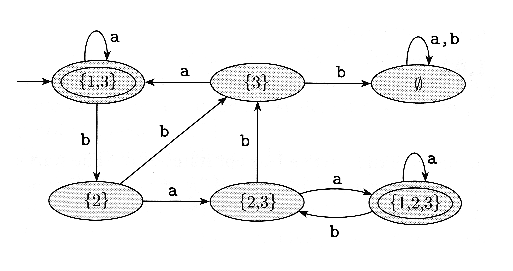
\includegraphics[height=20mm]{images/nfa3-dfa.eps}
\end{center}

Consider input strings $bba$, $baa$, and $a$.
\es

\bs{Regular Languages \& NFAs}
\vspace{.5in}
\begin{center}
\fbox{{\bf Theorem:} A language is regular if and only if some NFA recognizes it}
\end{center}

{\bf Proof Sketch:}
\begin{description}
\item[If a language is regular then some NFA recognizes it.]
	By definition, if a DFA recognizes a language, then it is regular.  It follows that there will
	be some NFAs that are equivalent to the recognizing DFA.  Therefore, if a language
	is regular, then there will be some NFA that recognizes it.
\item[If some NFA recognizes a language then the language is regular.]
	Any NFA can be converted into an equivalent DFA.  By definition this DFA
	recognizes the same language as the NFA.  The language a DFA recognizes
	is regular.  This implies that if an NFA recognizes a language, then the language is
	regular.
\end{description}
\es


\bs{More on NFAs}
NFAs facilitate proofs by allowing an easier construction of machines that recognize
regular languages.

Let's revisit our regular operations.
\es

\bs{Union - NFA}
{\bf Theorem:} The class of regular languages is closed under the union operation.

{\bf Proof Sketch:} Let $N_1$ and $N_2$ be the NFAs that recognize the languages $A_1$ and
$A_2$, respectively, we can then construct an NFA $N$ that recognizes the language
$A_1 \cup A_2$ as follows:\footnote{Formal proofs of this and the following theorems 
appear in the text pp59ff 1st \& 2nd eds.}

\begin{center}
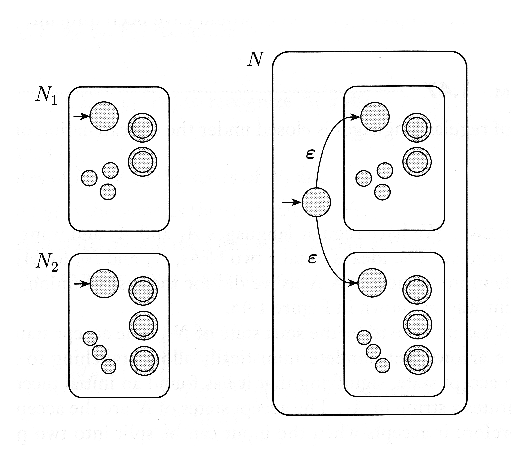
\includegraphics[height=50mm]{images/nfa-union.eps}
\end{center}
\es

\bs{Concatenation - NFA}
{\bf Theorem:} The class of regular languages is closed under the concatenation operation.

{\bf Proof Sketch:} Let $N_1$ and $N_2$ be the NFAs that recognize the languages $A_1$ and
$A_2$, respectively, we can then construct an NFA $N$ that recognizes the language
$A_1 \circ A_2$ as follows:

\begin{center}
\includegraphics[height=50mm]{images/nfa-concat.eps}
\end{center}
\es

\bs{Star - NFA}
{\bf Theorem:} The class of regular languages is closed under the kleene closure operation.

{\bf Proof Sketch:} Let $N_1$ be the NFA that recognizes the language $A_1$, we can then construct an NFA $N$ that recognizes the language
$A_1^*$ as follows:

\begin{center}
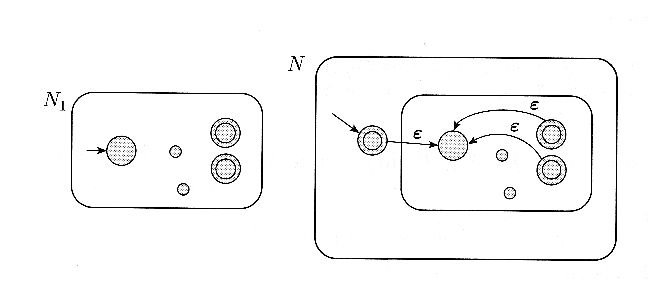
\includegraphics[height=40mm]{images/nfa-kleene.eps}
\end{center}
\es

\bs{Nonregular Languages}
Are there languages that FAs cannot recognize? Yes!

The prototypical 
language in this class of nonregular languages is the language 
\[
\{0^n 1^n  \mid 0,1 \in \Sigma \mbox{ and } n \ge 0 \}.
\]
The problem with this language is that the FA has to keep track of $i$ $0$'s
and make sure that for every  string in the language there are corresponding number
of $i$ $1$'s.

For the general case FAs cannot perform this task.

Can we prove this? Yes, the {\bf \em pumping lemma}.


\es

\bs{The Pumping Lemma}
The pumping lemma is based on the fact that if we pick a string with more symbols in it
than there are states then there has to be a loop in the sequence of states.  
Given this loop we can then walk around this loop as many times as we please
and for regular languages the strings generated are members of the original language
of the machine.  It is interesting to observe that for nonregular languages this
pumping does not work!  This gives us a way to prove that  a language is not
regular using contradiction.
\es


\bs{The Pumping Lemma}

{\bf Thereom (The Pumping Lemma):}  If $A$ is a regular language,
then there is a number $p$ (the {\bf\em pumping length}) where,
if $s$ is any string in $A$ of length at least $p$, then $s$ may be divided into
three pieces, $s = xyz$, such that
\begin{enumerate}
\item for each $i \ge 0, xy^iz \in A$,
\item $\mid y\mid > 0$, and
\item $\mid xy \mid \le p$.
\end{enumerate}
\begin{center}
\includegraphics[height=40mm]{images/nfa-pumping.eps}
\end{center}
\vspace{.2in}
\es

\bs{PL - Example}
\begin{center}
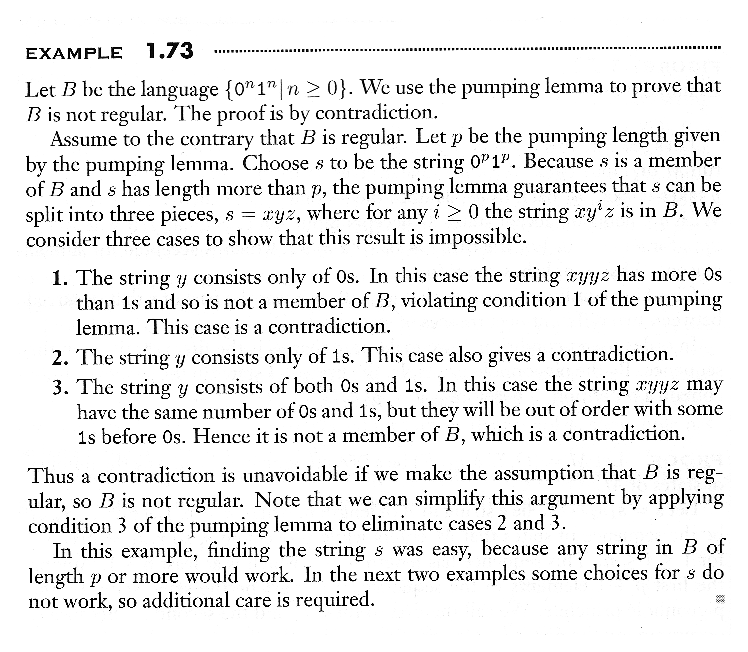
\includegraphics[height=70mm]{images/proof-pumping.eps}
\end{center}
\es

\bs{Proof Tools}
The material we have developed up to this point gives us the following tools to prove
properties of languages:
\begin{itemize}
\item In order to prove that a language is regular we construct a FA (either DFA or NFA since they are equivalent) that recognizes the language.
\item In order to prove that a language is nonregular, we assume that it is regular
and then show that this assumption leads to a contradiction in the pumping lemma.
\end{itemize}
\es

\bs{Assignment}

Assignment \#1 -- see website

\es
\end{document}
%%%%%%%%%%%%%%%%%%%%%%%%%%% end of template1.tex %%%%%%%%%%%%%%%%%%%%%%%%%%%%%%%%

